\chapter{非功能性需求}
\section{系统架构要求}
系统的构件图如图~\ref{fig:goujian}~所示。
\begin{figure}[htbp]
    \centering
    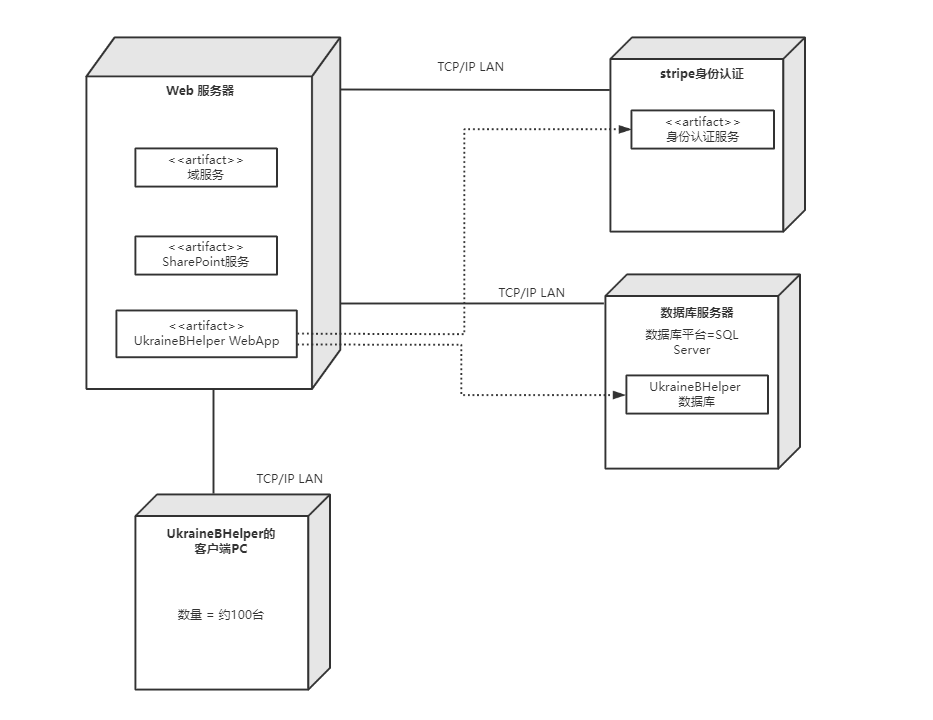
\includegraphics[width=\textwidth]{ch6/goujian.png}
    \caption{系统构件图}\label{fig:goujian}
    \vspace{\baselineskip} % 表示图与正文空一行
\end{figure}
系统的架构图如图~\ref{fig:jiagou}~所示。
\begin{figure}[htbp]
    \centering
    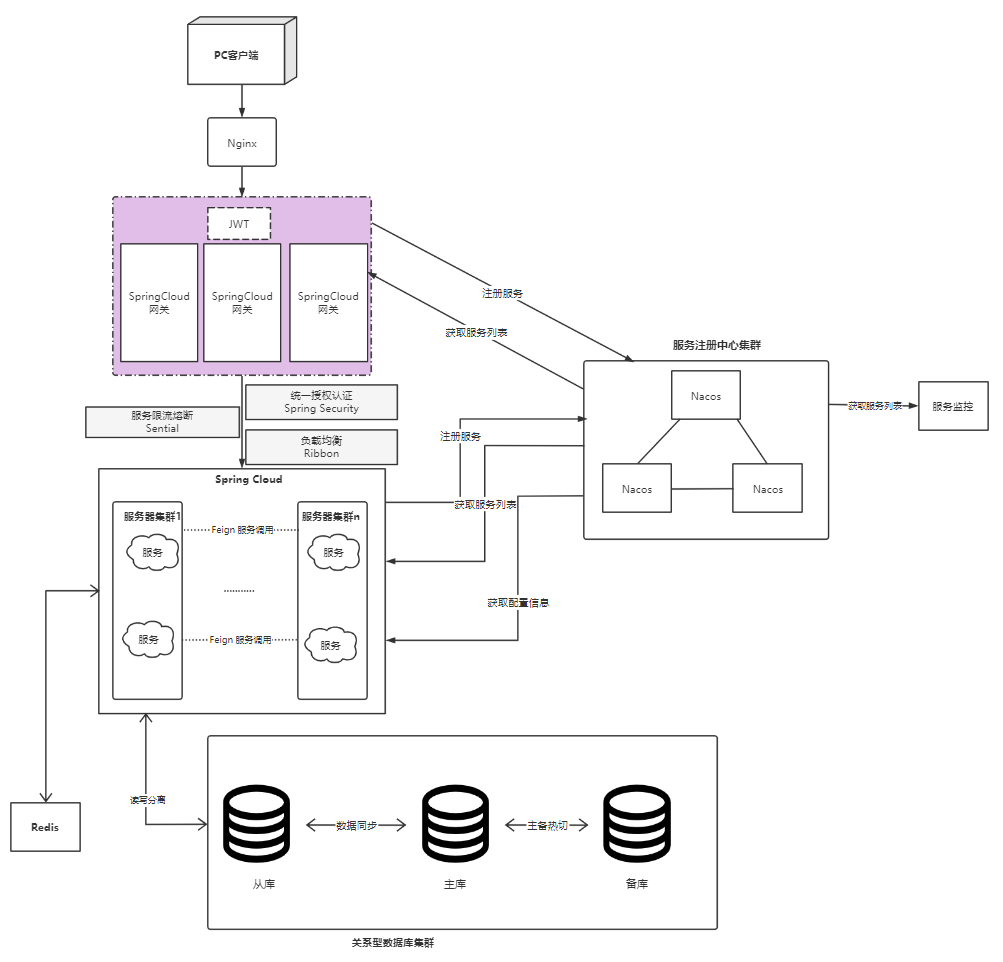
\includegraphics[width=\textwidth]{ch6/bushu.png}
    \caption{系统部署图}\label{fig:jiagou}
    \vspace{\baselineskip} % 表示图与正文空一行
\end{figure}
\section{接口}
\textbf{待填写}
\section{安全性}
\begin{enumerate}
    \item 房主发布房源必须要进行身份认证,已保障难民的安全。对于房主的身份信息保证保密。
    \item 可以做到维持,不过用户更换客户机的时候需要重新登录(已认证则不必再次认证)。
    \item 难民有举报功能,要是需要使用此功能,需要登录。
    \item 设计过程需要充分的考虑到恶意代码的非法入侵行为,保证达到安全可靠性最高。
\end{enumerate}
\section{性能}
\subsection{时间需求}
\begin{enumerate}
    \item 查询时间的最长等待时间不超过2秒
    \item 更新信息的最长时间不超过3秒
    \item 数据上传和下载时间最长不超过3秒
\end{enumerate}
\subsection{空间需求}
\begin{enumerate}
    \item 支持的终端数不超过10000
    \item 支持并行操作的使用者不超过5000
    \item 记录处理数:10000
\end{enumerate}
\section{设计约束}
\begin{enumerate}
    \item 建议硬盘:128GB 或更高
    \item 建议内存:256MB 或更高
    \item 建议CPU:1.4GHZ 或更高
    \item 网络环境:广域网/局域网。有线网络访问速度更快。
\end{enumerate}
\section{界面}
\textbf{待填写}